\section{Homogenization}
\begin{frame}{Variable Properties With a Single Material}
    \begin{itemize}
        \item How can we vary the material properties with one material? Vary the microstructure
              geometry.
        \pause 
        \begin{figure}
            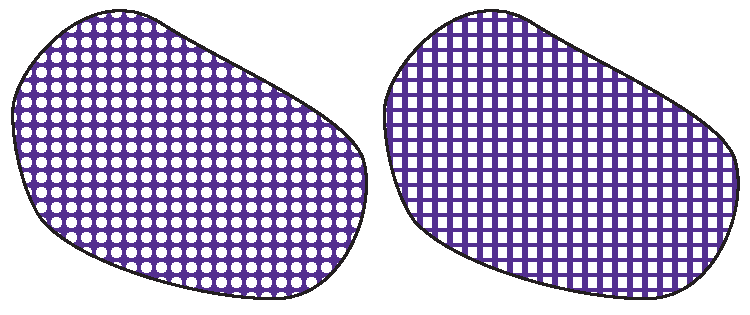
\includegraphics[width=.65\textwidth]{Images/two_patterns.pdf}
        \end{figure}
        \pause \item Gives different effective, ``homogenized,'' material properties:
        \begin{figure}
            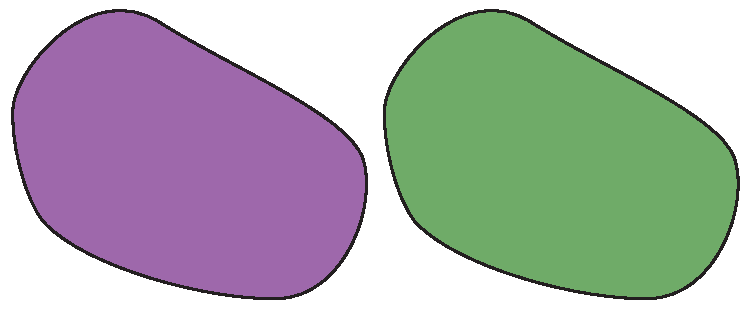
\includegraphics[width=.65\textwidth]{Images/two_materials.pdf}
        \end{figure}
    \end{itemize}
\end{frame}

\begin{frame}{Homogenized Elasticity Tensor}
    \begin{itemize}
\item Recall: material properties (elasticity tensor) tell us how strain maps to
    stress.
\item Intuitively: homogenized elasticity tensor tells us how the {\bf average} strain
    ``around'' a point maps to the {\bf average} stress.
\item Can't spatially average the properties!
    \begin{figure}
        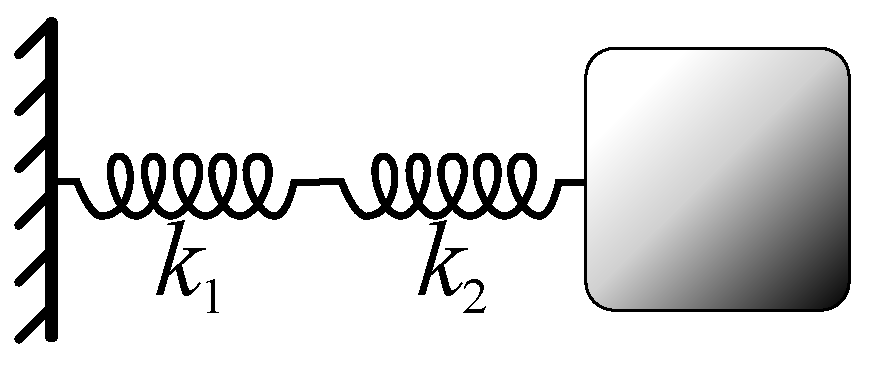
\includegraphics[width=.50\textwidth]{Images/SpringsInSeriesWiki.pdf}
    \end{figure}
    $$k^H = \frac{1}{\frac{1}{k_1} + \frac{1}{k_2}} \ne \frac{1}{2}\left(k_1 +
    k_2\right)$$
    \end{itemize}
\end{frame}

\begin{frame}{Homogenized Elasticity Tensor}
    \begin{itemize}
        \item To use nice mathematical tools (periodic homogenization), restrict
            to microstructures given by tiled base cells. 
            \begin{figure}
                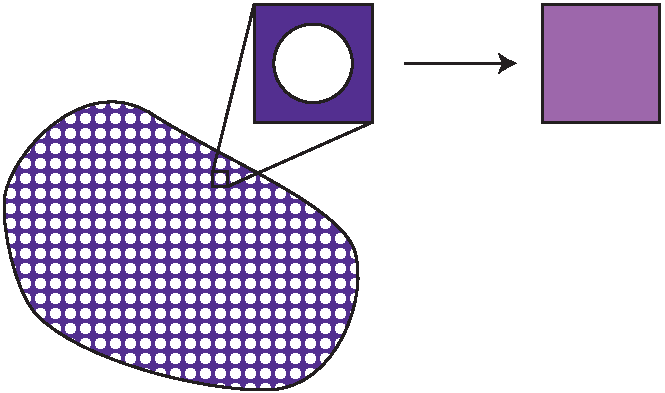
\includegraphics[width=.50\textwidth]{Images/cell_homogenize.pdf}
                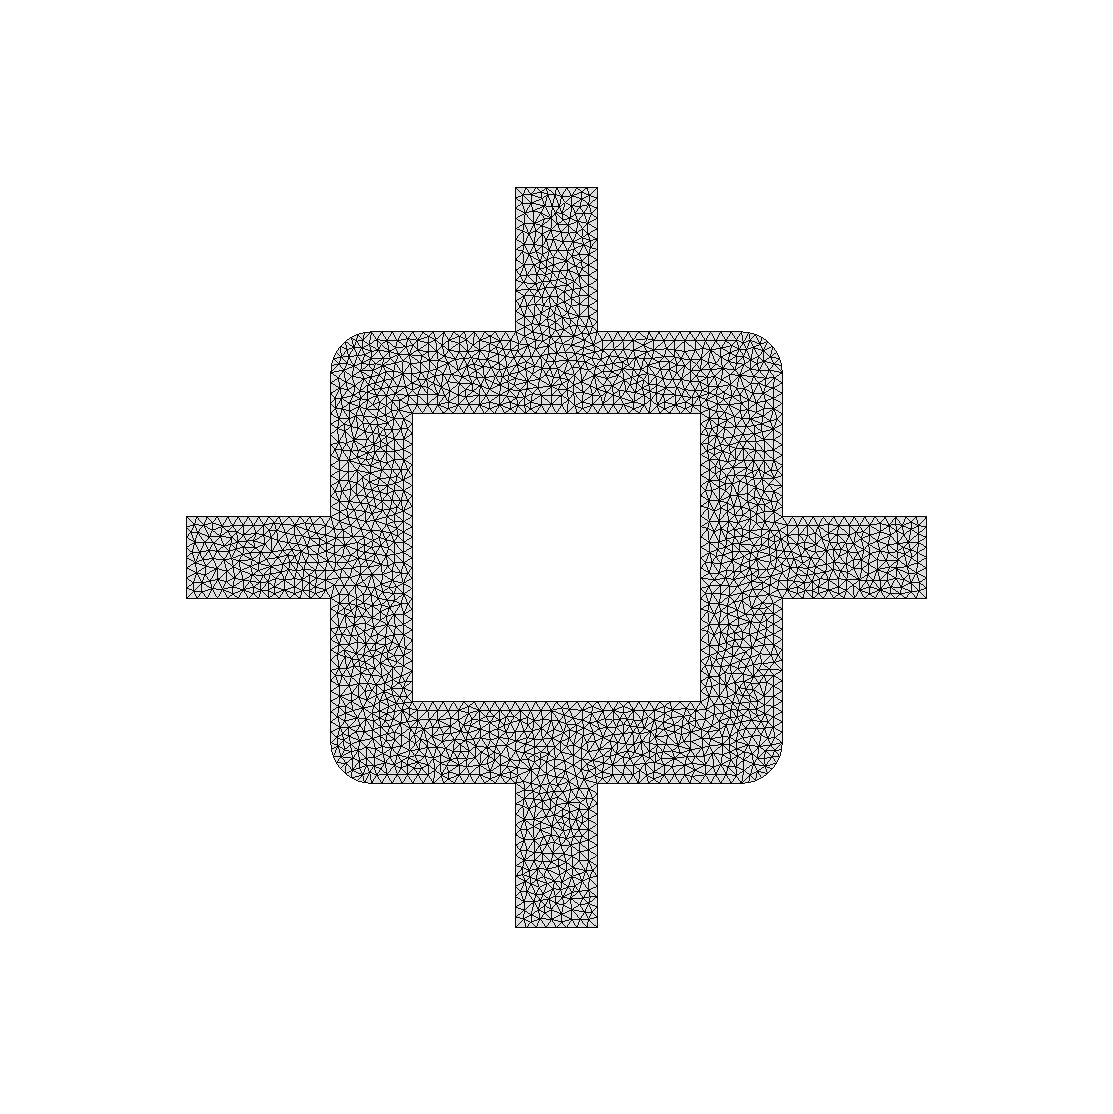
\includegraphics[width=.40\textwidth]{Images/base.png}
            \end{figure}
        \item General idea: for all possible average strains over the cell, compute the
              average stress.
    \end{itemize}
\end{frame}

\begin{frame}{Strain Tensor Basis}
    \begin{itemize}
        \item Linearity of stress-strain relationship saves us: we only need to consider 3
    ``basis strain tensors'' in 2D: 2 axis-aligned stretches and 1 shear.
    \begin{figure}
        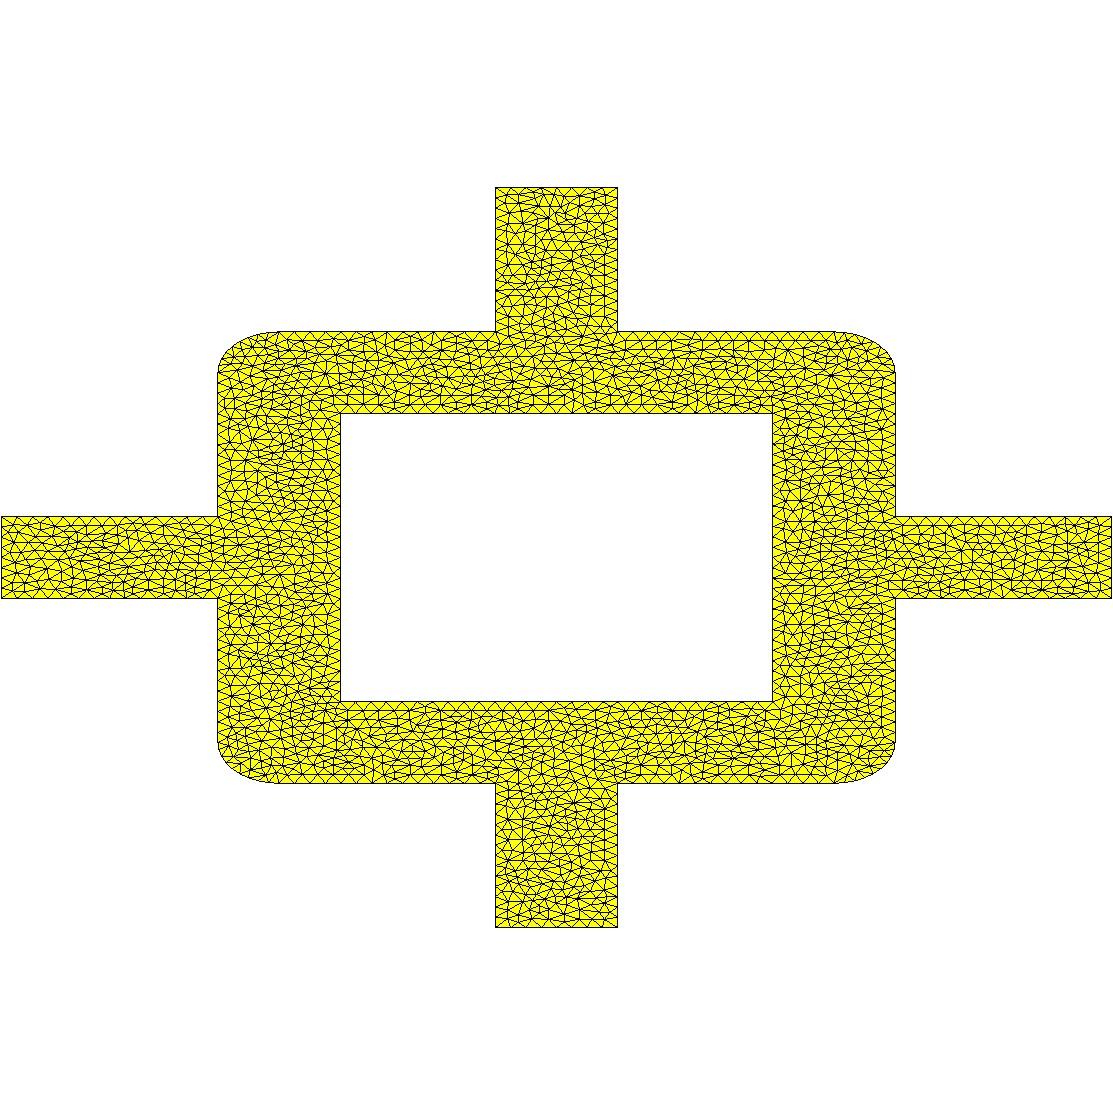
\includegraphics[width=.25\textwidth]{Images/cstrain_x.png}
        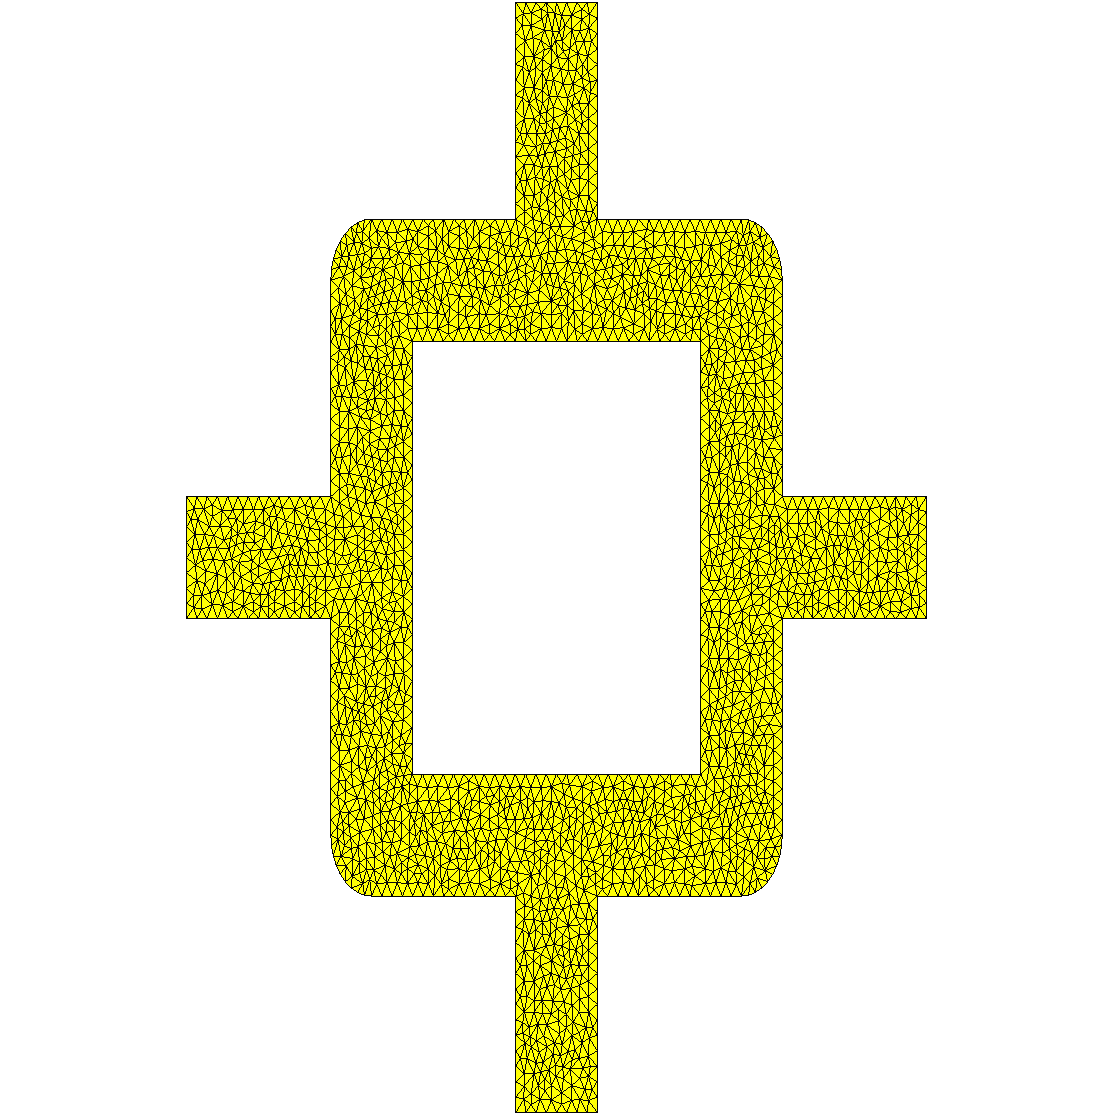
\includegraphics[width=.25\textwidth]{Images/cstrain_y.png}
        
\includegraphics[width=.25\textwidth]{Images/cstrain_shear.png}
    \end{figure}
    \begin{figure}
        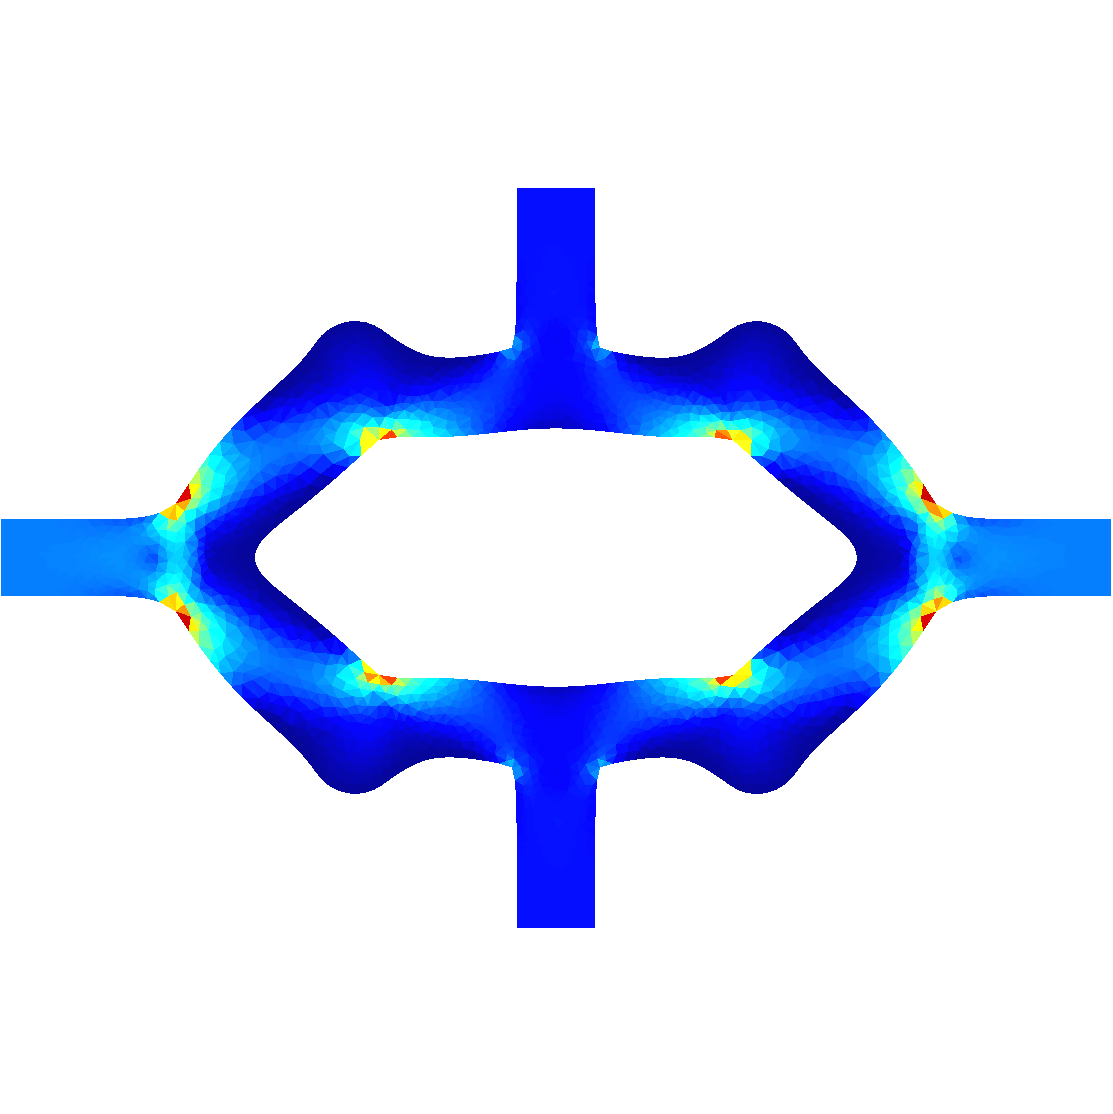
\includegraphics[width=.25\textwidth]{Images/disp_x.png}
        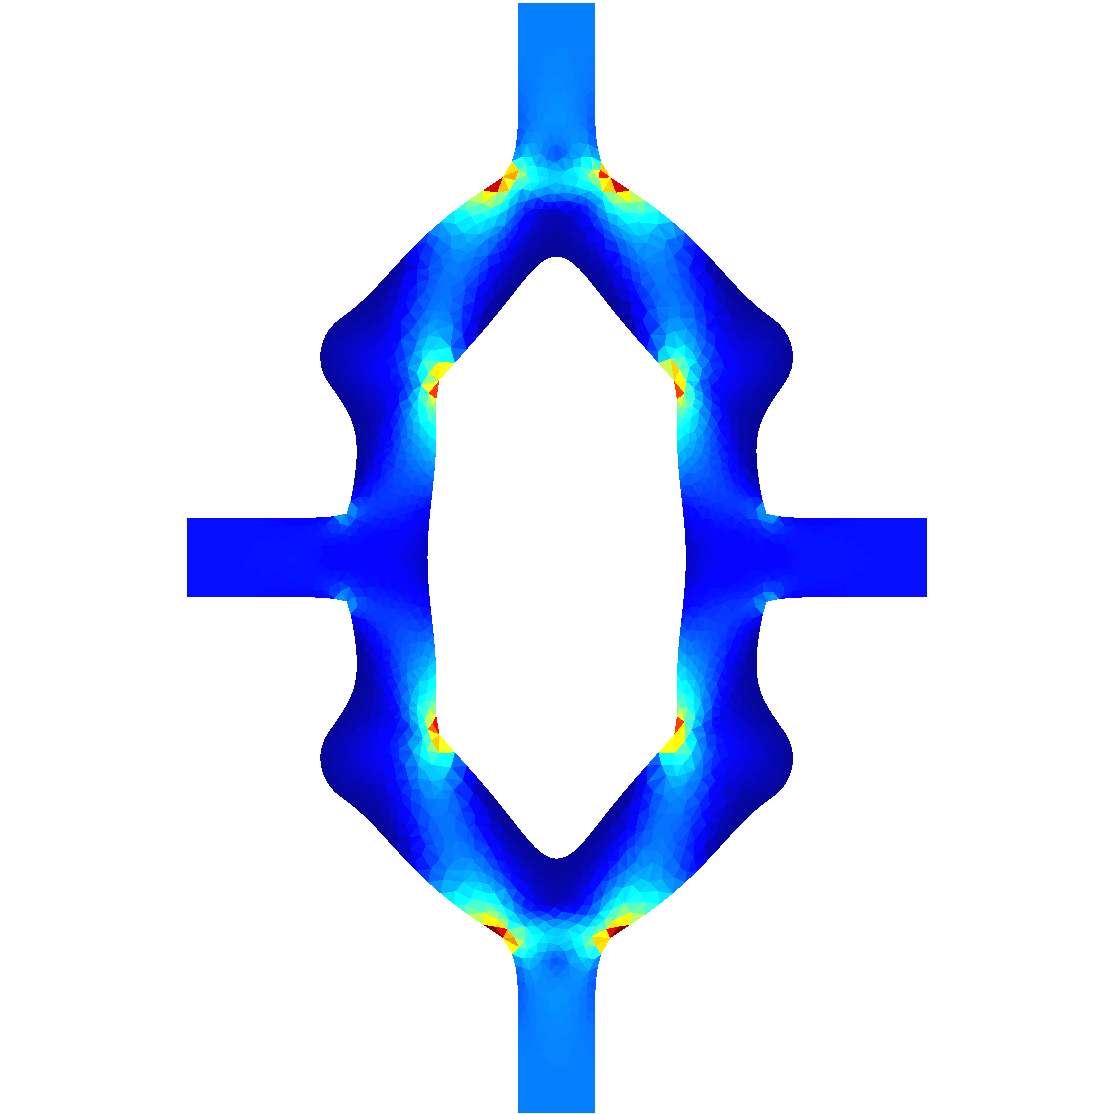
\includegraphics[width=.25\textwidth]{Images/disp_y.png}
        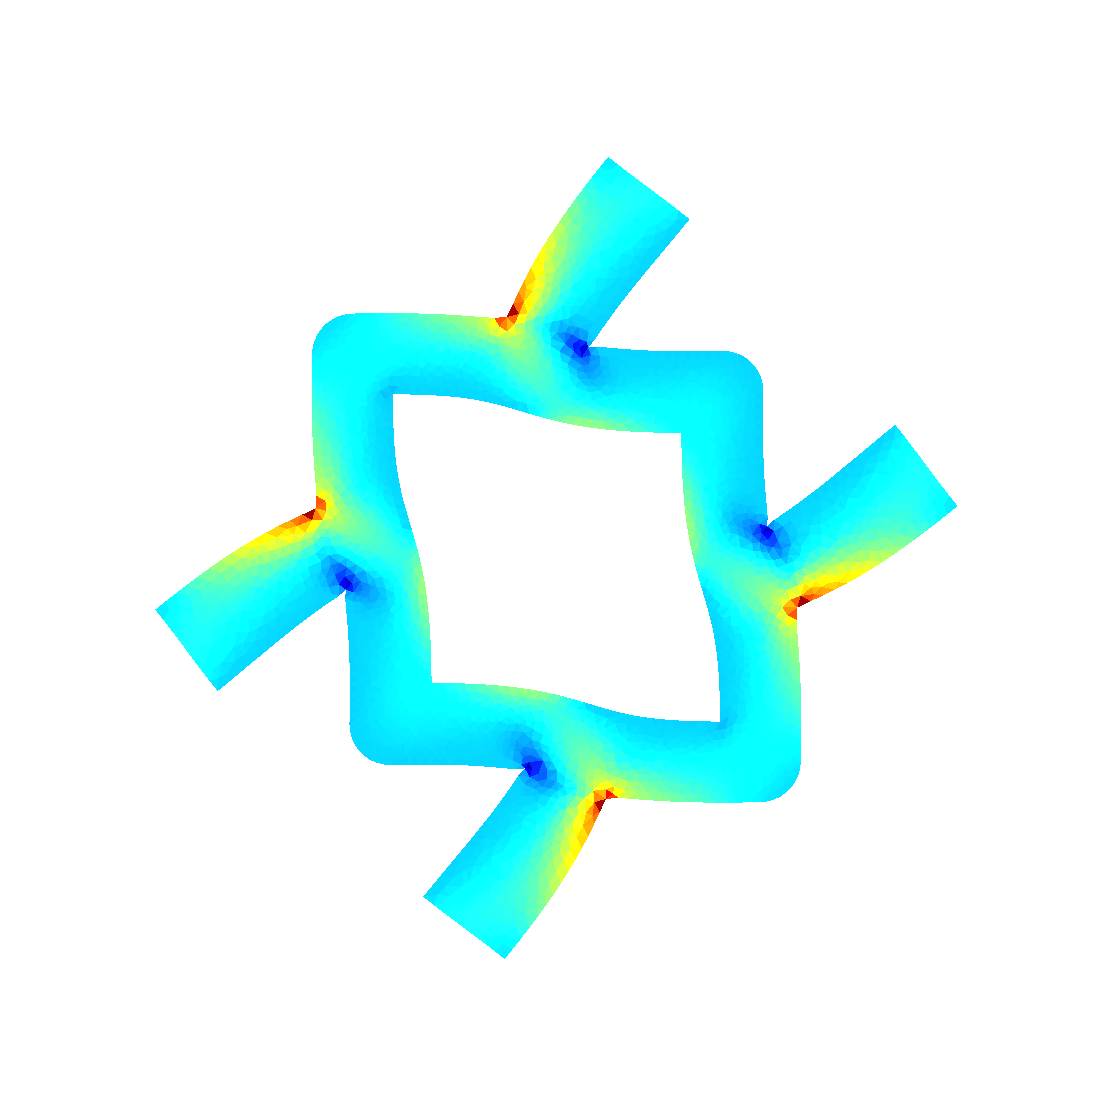
\includegraphics[width=.25\textwidth]{Images/disp_shear.png}
    \end{figure}
    \end{itemize}
\end{frame}

\begin{frame}{Computing the Homogenized Elasticity Tensor}
    \begin{figure}
        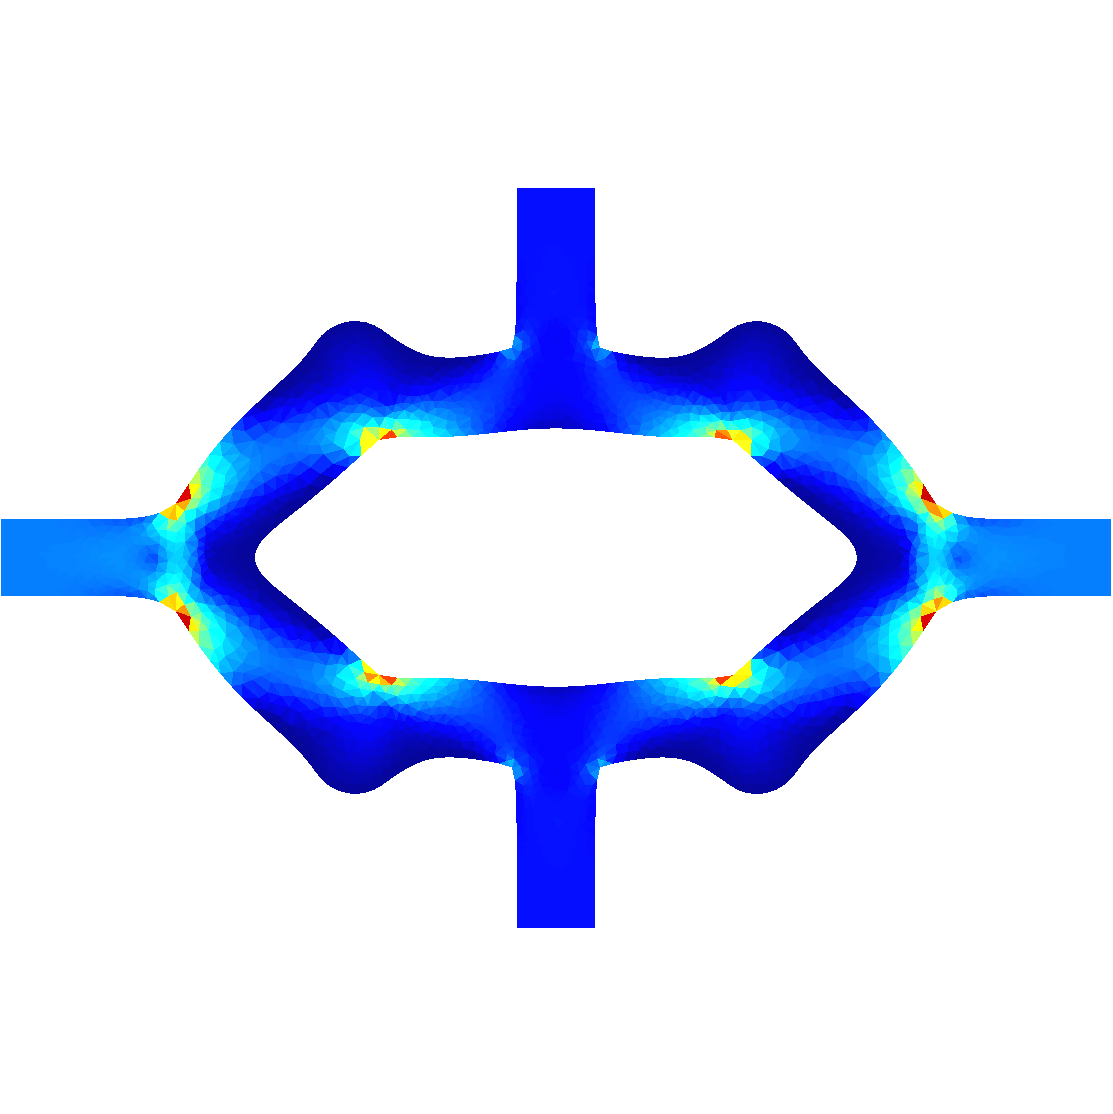
\includegraphics[width=.25\textwidth]{Images/disp_x.png}
        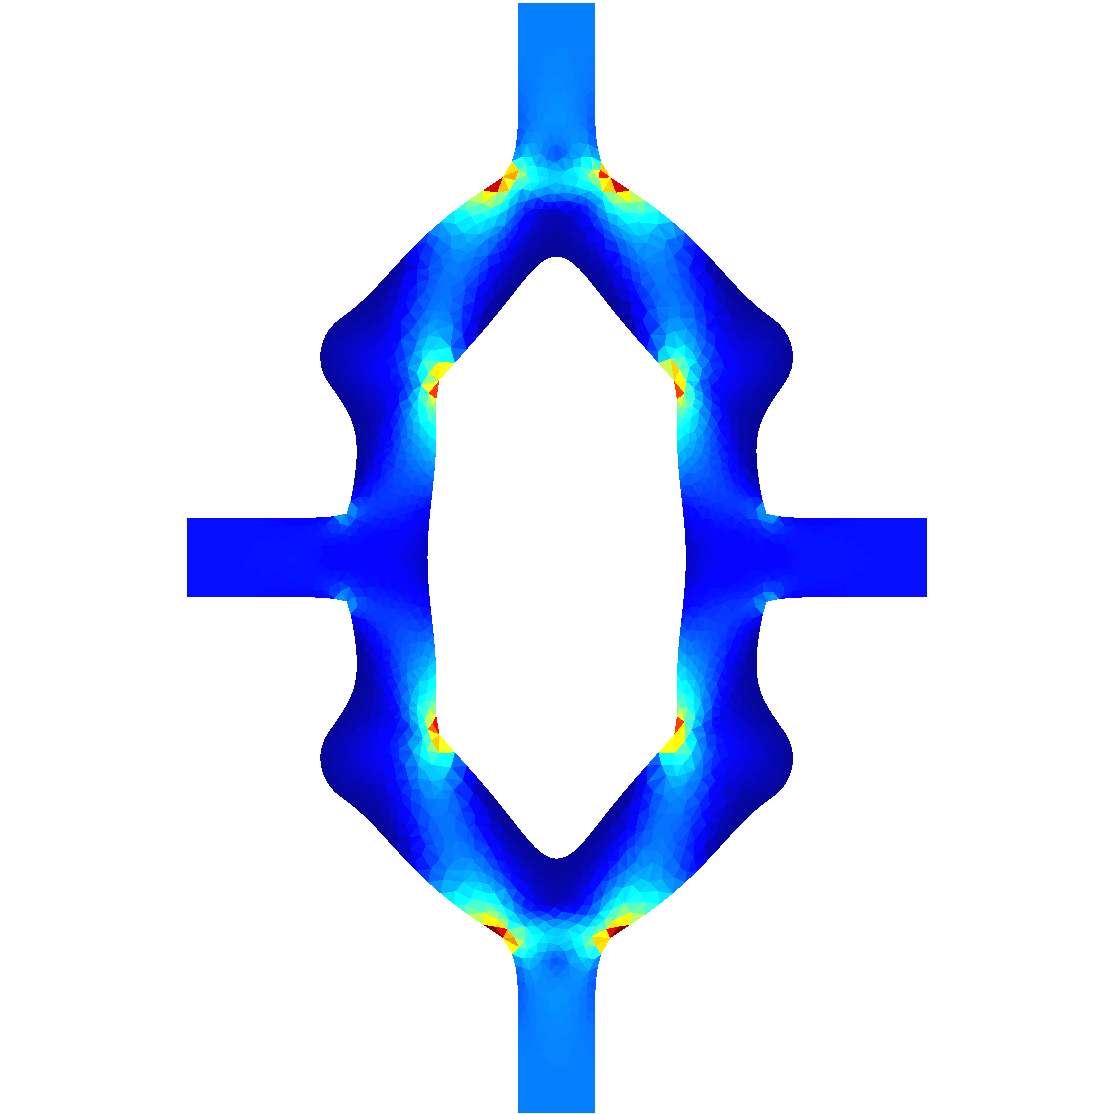
\includegraphics[width=.25\textwidth]{Images/disp_y.png}
        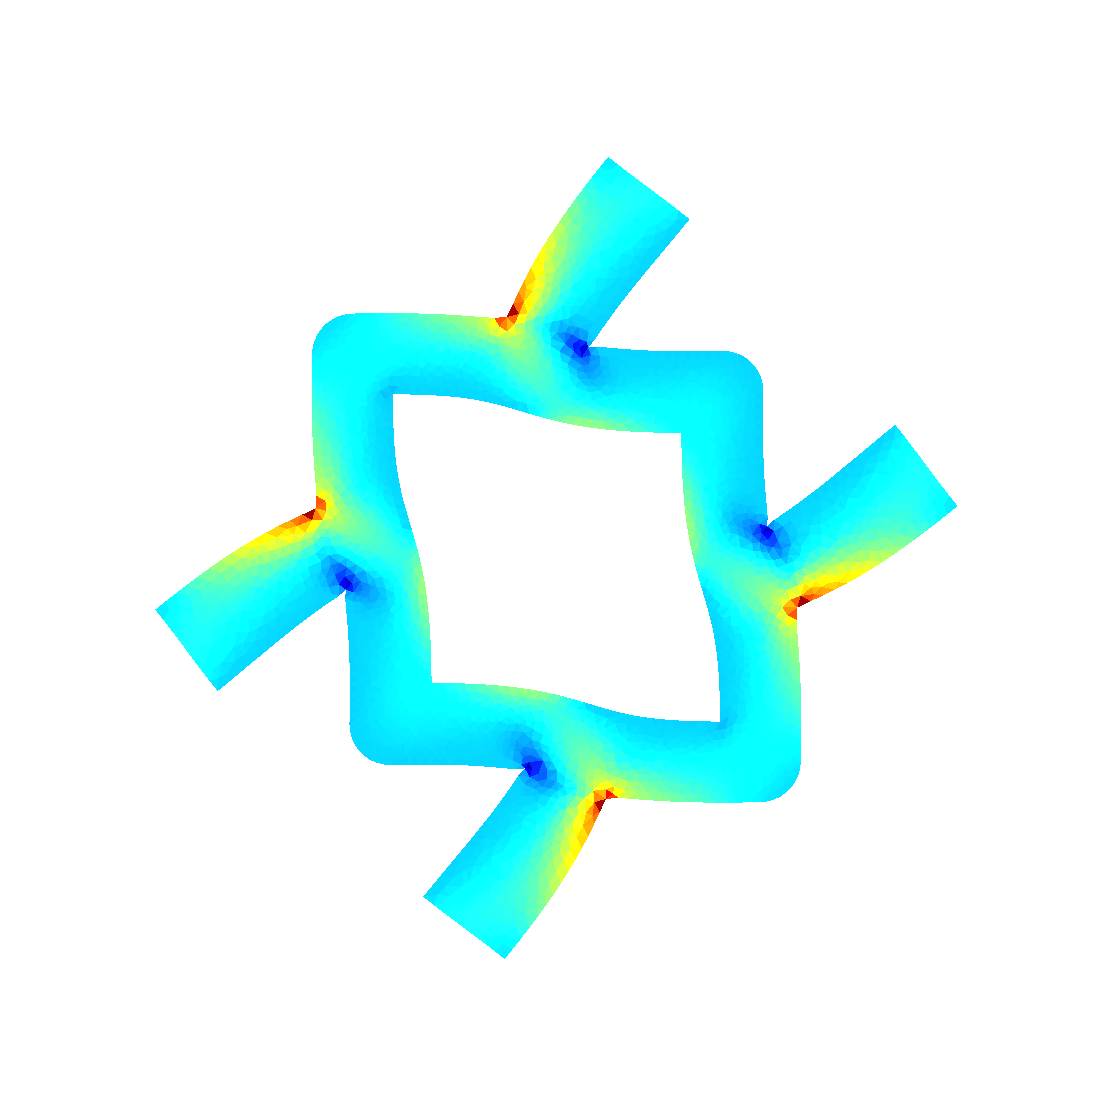
\includegraphics[width=.25\textwidth]{Images/disp_shear.png}
    \end{figure}
    \begin{itemize}
        \item For each constant strain basis tensor:
        \begin{itemize}
            \item Impose the average constant strain and compute how the geometry
                  actually deforms
            \item Average the stress tensor over the cell
            \item Store flattened average stress tensor in a column of the
                  flattened elasticity tensor.
        \end{itemize}
    \end{itemize}
\end{frame}

\begin{frame}{Computing the Homogenized Elasticity Tensor}
    \begin{figure}
        
\includegraphics[width=.20\textwidth]{Images/cell.pdf}
    \end{figure}
    \begin{align*}
         -\nabla \cdot (C^\text{base} : [e({\bf w}^{ij}) + e^{ij}]) = {\bf 0} & \quad \text{in } \omega \\
    {\bf \hat n} \cdot (C^\text{base} : [e({\bf w}^{ij}) + e^{ij}]) = {\bf 0} & \quad \text{on } \partial \omega \setminus \partial Y \\
        {\bf w}^{ij}({\bf y})\ Y \text{-periodic} & \\
        \int_\omega \! {\bf w}^{ij}({\bf y})  \, \mathrm{d} {\bf y} =  {\bf 0}, 
    \end{align*}
    \begin{equation*}
        \label{eqn:Eh}
    C^H_{ijkl} = \frac{1}{|Y|} \int_Y C^\text{base}_{ijpq} [e({\bf w}^{kl})] + e^{ij}]_{pq} \, \mathrm{d} {\bf y}
    \end{equation*}
    \begin{itemize}
        \pause \item As cell size shrinks to zero, the microstructure simulation
            converges to a homogenous simulation with $C^H$
   \end{itemize}
\end{frame}
